\datos{color}{}{}
\section{Robots}
\subsection{\textit{Shakey}}
%\addcontentsline{toc}{section}{Ejercicio 1}

\textit{Shakey}, concebido por el \textit{Stanford Research Institute} (\textit{SRI}) durante los años
1966–1972, Figura \ref{shakey}, fue el primer robot móvil capaz de razonar sobre sus acciones e 
implementar una arquitectura en capas. Integraba visión artificial, planificación simbólica, 
navegación y control en un único sistema, apoyándose en una cámara de televisión, un telémetro
para medir distancias y varios sensores de contacto conectados al ordenador central 
\textit{PDP-10}. Fue pionero en inteligencia artificial y robótica cognitiva y podía moverse por 
habitaciones, empujar objetos y planificar rutas. \\

\begin{comment}
\begin{wrapfigure}{r}{0.3\textwidth}
    \centering
    \vspace{-10pt}
    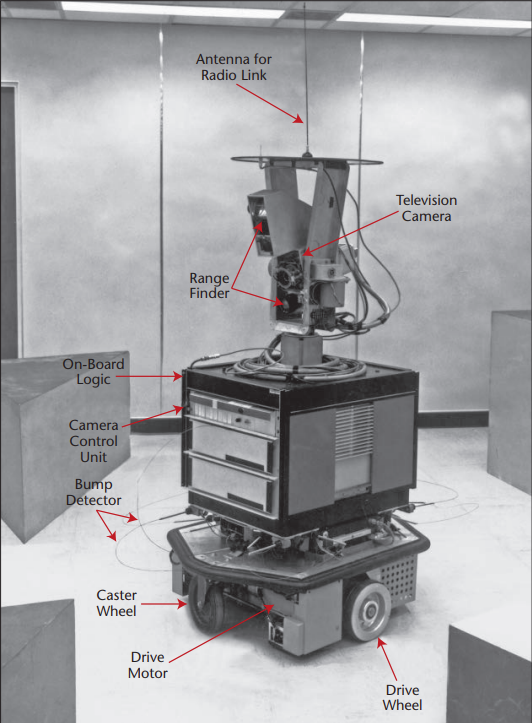
\includegraphics[width=0.25\textwidth]{Images/shakey.png}
    \caption{\textit{Shakey}.}
    \label{shakey}
    \vspace{-10pt}
\end{wrapfigure}
\end{comment}

Sus usos principales fueron la investigación en inteligencia artificial, robótica cognitiva 
y el desarrollo de planificación simbólica (\textit{STRIPS}) y experimentos de percepción, navegación y 
razonamiento. De hecho, la investigación realizada por el \textit{SRI} con \textit{Shakey}
obtuvo como resultado el algoritmo de búsqueda A* y los primeros algoritmos de
navegación y visión artificial. \\

La arquitectura de \textit{Shakey} seguía un modelo completamente centralizado y jerárquico, 
estructurado en capas de percepción, representación del mundo, planificación y ejecución, 
como se observa en la Figura 5 de \cite{Shakey}. Cada una de estas capas correspondía a un 
módulo específico del sistema de control y el flujo seguía la descomposición vertical clásica: 
sensación $\rightarrow$ percepción $\rightarrow$ modelo del mundo $\rightarrow$ planificación 
$\rightarrow$ acción. \\

La capa de ejecución estaba formada por las acciones de bajo nivel, que interactuaban 
directamente con el \textit{hardware}, y por las acciones intermedias basadas en tablas de 
Markov, responsables de comportamientos reactivos persistentes. La capa de planificación 
correspondía a \textit{STRIPS}, el planificador simbólico encargado de generar secuencias de 
acciones para alcanzar objetivos complejos. Finalmente, la capa de representación del mundo 
estaba asociada a \textit{PLANEX}, que supervisaba la ejecución del plan, detectaba errores, 
replanificaba cuando era necesario y mantenía la coherencia entre el estado simbólico y el 
estado real del entorno. \\

\begin{wrapfigure}{r}{0.32\textwidth}
    \centering
    \vspace{-10pt}
    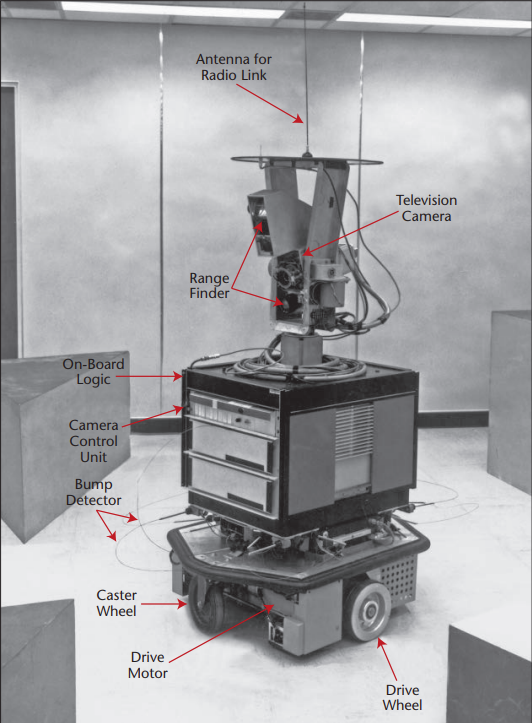
\includegraphics[width=0.28\textwidth]{Images/shakey.png}
    \caption{\textit{Shakey}.}
    \label{shakey}
    \vspace{-10pt}
\end{wrapfigure}

Shakey utilizaba un sistema de locomoción basado en dos ruedas motrices diferenciales (\textit{drive wheel}) 
y una rueda pasiva (\textit{caster wheel}) para mantener la estabilidad. El movimiento se controlaba variando
la velocidad relativa de las dos ruedas motrices, permitiendo avanzar, retroceder y girar 
sobre su propio eje.


\subsection*{Referencias}
\cite{Shakey} \fullcite{Shakey}.

\begin{comment}
\begin{figure}[H]
    \begin{center}
    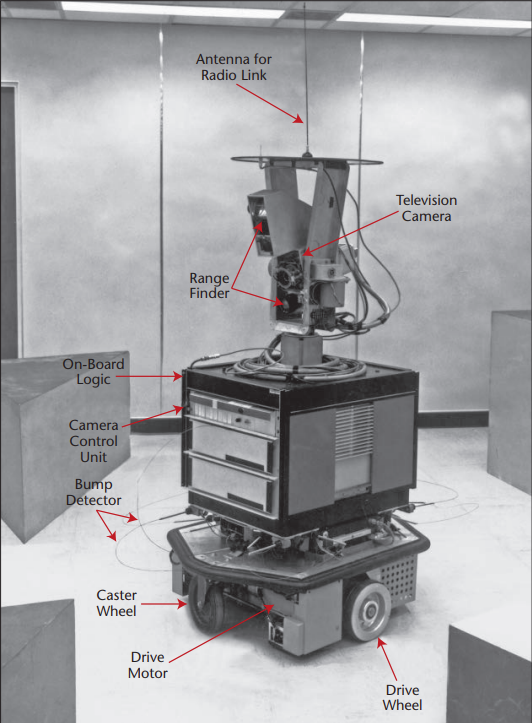
\includegraphics[scale=0.2, angle=0]{Images/shakey.png}
    \caption{\label{shakey}\textit{Shakey}.}
    \end{center}
\end{figure}
\end{comment}
